\chapter{La naissance et l’évolution de CujasNum (2001 – 2024)}

\lettrine{L}a numérisation des documents anciens demande au préalable une réflexion poussée \enquote{portant sur les choix techniques comme intellectuels} \footcite{joannic-setaEtudePrealableOperation1999}. Pour la Bibliothèque Cujas, l'opération de numérisation représente en effet un puissant levier pour valoriser scientifiquement ses collections patrimoniales et en élargir durablement l'accès. La bibliothèque Cujas fait partie des premières bibliothèques françaises à avoir développé une bibliothèque numérique afin de valoriser ses collections patrimoniales. Historiquement, les bibliothèques numériques ne répondaient pas aux mêmes enjeux qu'aujourd'hui: à l'origine, elles se réduisaient le plus souvent à une exposition de fichiers PDF \footcite{dipietroProduireContenusDocumentaires2014}. Cette approche tranche avec celle contemporaine, qui les appréhende désormais comme une véritable extension de la bibliothèque physique, permettant de valoriser les fonds sous diverses formes, telles que des expositions virtuelles, des parcours guidés, des articles scientifiques ou des billets de blog \footcite{bermesWebSemantiqueBibliotheque2013}. Au début des années 2000, le paysage technologique offrait un choix relativement restreint de solutions logicielles. Dans ce contexte, la bibliothèque Cujas fit le choix de concevoir son infrastructure sous XTF (eXtensible Text Framework), un outil open-source développé par l'Université de Californie, très prisé dans le monde anglo-saxon et dont la communauté d'utilisateurs louait alors la grande robustesse \footnote{Voir l'\ref{annexe_A_rapport_audit}.}. Néanmoins, l'un des inconvénients majeurs d'XTF réside dans son architecture de données dite \enquote{à plat}. Cette absence de granularité empêchait l'intégration de types de documents exigeant une arborescence complexe, à l'instar des documents périodiques ou des fonds d'archives \footnote{Voir l' \ref{annexe_A_rapport_audit}.}.

\section[Bibliothèque numérique]{Histoire de la bibliothèque numérique}
L'élaboration de la bibliothèque numérique CujasNum ne s'est pas faite de manière linéaire, mais résulte d'une succession de jalons éditoriaux et scientifiques qui ont progressivement défini l'identité numérique de l'établissement.

\subsection{Les balbutiements de la numérisation à Cujas (2001-2007)}
Malgré la richesse des collections conservées dans la réserve de la Bibliothèque Cujas, celle-ci ne rencontre pas immédiatement le succès escompté auprès des usagers. Frédérique Joannic-Seta corrobore ce constat, attribuant ce manque d'attrait à \enquote{ses difficultés d'ouverture de consultation qui entraînent une faible utilisation au regard de sa réelle richesse} \footcite{joannic-setaEtudePrealableOperation1999}. Par ailleurs, de nombreux volumes se trouvent alors en mauvais état, ayant subi aussi bien des \enquote{inondations exceptionnelles dans les magasins que des dégradations quotidiennes suscitées par les manipulations et les conditions de conservation, longtemps médiocres} \footcite{joannic-setaEtudePrealableOperation1999}. 

En 1998, soucieuse de valoriser cette réserve patrimoniale, la Bibliothèque Cujas décide d'engager la numérisation de ses collections. Son choix est dicté par \enquote{un souci de conservation des documents par la mise à disposition des lecteurs d'un support de substitution de qualité} \footcite{joannic-setaEtudePrealableOperation1999}. Le second objectif vise à faciliter l'accès aux fonds pour permettre aux lecteurs \enquote{une meilleure appropriation du texte en leur proposant des facilités de reproduction} \footcite{joannic-setaEtudePrealableOperation1999}. 

L'un des premiers chantiers de numérisation de la Bibliothèque Cujas remonte aux années 2000 et 2001. Durant cette phase pionnière, l'établissement fait numériser 17 titres représentant environ 22 volumes, une tâche externalisée auprès de la société Safig \footcite{2006ProgrammeNumerisation}. La bibliothèque commande alors une numérisation \enquote{en mode image, avec une navigation grâce à la pagination}\footnote{\nameref{annexe_A_rapport_audit}.}. Séduite par l'offre du prestataire qui propose de prendre en charge l'hébergement et la diffusion en ligne des documents sur ses propres serveurs, la Bibliothèque Cujas choisit de lui déléguer l'ensemble de cette chaîne de stockage et de mise à disposition. 

Cette stratégie se révèle désastreuse : la société est victime d'une attaque sur ses serveurs, entraînant la perte irrémédiable d'une majeure partie des documents numérisés. Face à ce sinistre, la bibliothèque s'efforce de récupérer ce qu'elle peut \footcite{2006ProgrammeNumerisation}. Le prestataire Safig restitue ce qui lui reste \enquote{sous forme de CD-ROM}. À la réception des CD-ROM, le personnel de Cujas tente de déterminer s'il est possible \enquote{de réutiliser du contenu}. Cette tentative de sauvetage s'avère toutefois vaine: les fichiers réceptionnés se révèlent irrécupérables, voire corrompus pour certains, contraignant l'établissement à prendre la décision de renumériser intégralement le corpus \footnote{\nameref{annexe_A_rapport_audit}.}.

Le choix de la Bibliothèque Cujas est d'orienter d'emblée la valorisation de son contenu vers \enquote{un lectorat universitaire de haut niveau} \footcite{balley4ExempleMediation2012}. Noëlle Balley, alors chargée de mission pour le patrimoine et future responsable du département des Monographies de la Bibliothèque Cujas, et son adjoint de l'époque, Sébastien Dalmon, attribuent cette volonté à la spécialisation extrême du fonds: à leurs yeux, ce contenu \enquote{souvent aride} s'avère peu propice à une \enquote{valorisation orientée vers le grand public} \footcite{balley4ExempleMediation2012}. L'établissement privilégie donc des corpus spécifiquement sélectionnés pour ce public académique, en mettant à sa disposition des \enquote{outils facilitant leur travail sur les textes}\footcite{balley4ExempleMediation2012}. Toutefois, ils soulignent que malgré les moyens mis en oeuvre pour s'adresser à ce lectorat élitiste, il convient de ne pas \enquote{négliger le grand public} \footcite{balley4ExempleMediation2012}.

\subsection{La liste Pfister-Roumy}
Afin de valoriser la richesse de ce patrimoine, la Bibliothèque Cujas conçoit le projet de développer sa propre bibliothèque numérique, une ambition émergeant en même temps que la numérisation des cours de Jean Carbonnier \footcite{2006ProgrammeNumerisation}. À l'origine, l'établissement souhaite s'insérer dans une dynamique nationale en postulant à l'appel à projets de Persée, dans l'espoir de devenir un pôle de réplication \footcite{2006ProgrammeNumerisation}. C'est dans cette perspective que la bibliothèque acquiert un scanner Kirtas destiné à créer sa chaîne de traitement interne. Bien que cette candidature n'ait finalement pas été retenue, elle sera le point de départ de la réflexion de la bibliothèque souhaitant capitaliser sur cette acquisition \footcite{2007RefonteProgramme}. 

La direction de la bibliothèque Cujas change alors de stratégie.. Elle choisit de s'associer étroitement avec deux éminents  historiens du droit de la Faculté de Droit de Paris, les professeurs Laurent Pfister et Franck Roumy \footcite{2006ProgrammeNumerisation}. Cette collaboration inédite entre les professionnels des bibliothèques et les enseignants-chercheurs permet d'élaborer une première liste de référence scientifique, désignée plus tard sous le nom de \enquote{liste Pfister-Roumy} \footcite{2007RefonteProgramme}.

La numérisation de la collection Jean Carbonnier est la première opération de numérisation interne de la Bibliothèque Cujas. Elle a donc permis de tester \enquote{en grandeur réelle, la chaîne de numérisation qu'elle mettait en place pour son propre programme} \footcite{2007RefonteProgramme}. Face au succès de cette première numérisation, les équipes la réemploient au moment de son deuxième plus gros projet de numérisation, la liste \enquote{Pfister-Roumy}.

Contrairement au projet Carbonnier, ce nouveau projet ne se concentre plus sur des cours polycopiés, mais vise à numériser en priorité  les grands textes fondamentaux et les sources doctrinales de l'histoire du droit.

L'objectif de la liste Pfister-Roumy est de sélectionner des monographies et des périodiques issus \enquote{uniquement des collections de Cujas}. Cette sélection porte sur les \enquote{fondamentaux du droit à numériser en priorité} \footcite{2006ProgrammeNumerisation}. À l'origine, les deux professeurs recensent \enquote{471 titres fondamentaux pour la recherche en histoire du droit}, couvrant une vaste période allant du \enquote{XVe siècle au XXe siècle, soit 1462 volumes et 1 001 559 pages}\footcite{2006ProgrammeNumerisation}. À cet ensemble patrimonial, les professeurs adjoignent deux périodiques de référence: \enquote{Duvergier et le Bulletin des arrêts de la Cour de cassation (Chambre criminelle et Chambres civiles) jusqu'en 1950.}\footcite{2006ProgrammeNumerisation}. Ce projet est initialement pensé lors de la candidature de Cujas pour devenir pôle de réplication de Persée, se caractérise par des ambitions techniques élevées, reposant sur une \enquote{numérisation automatique non descriptive, en mode image océrisé, avec une recherche plein texte et la structuration documentaire à granularité fine, emploi de la DTD TEI, réalisée exclusivement en interne} \footcite{2006ProgrammeNumerisation}.

L'abandon de ce projet de réplication oblige la Bibliothèque Cujas à repenser son programme de numérisation, contraignant l'établissement à revoir à la baisse le nombre d'ouvrages sélectionnés. Le corpus initial est ainsi réduit, passant de 471 ouvrages à 436 ouvrages \footcite{2007RefonteProgramme}. En effet, à la même époque, la \ac{BNF} développe en parallèle un projet scientifique similaire, intitulé la liste Kerbrat. Élaborée sous la direction du professeur Yann Kerbrat et d'un groupe de quatorze universitaire, cette sélection a pour objectif \enquote{de créer une liste de références à partir des collections de la BNF} dans le domaine du droit \footcite{2007RefonteProgramme}. Dans un soucis d'optimisation des moyens financiers et de cohérence scientifique, une concertation étroite s'établit entre les deux institutions afin de coordonner leurs campagnes respectives et d'éviter les doublons. Ainsi, lorsque la Bibliothèque Cujas conserve un ouvrage identique à celui de la \ac{BNF}, il lui est néanmoins permis de le numériser, mais à la condition expresse de sélectionner une édition différente de celle de la \ac{BNF}. Certains titres, impossible à substituer par une autre édition, sont alors purement et simplement retirés de la liste de Cujas \footnote{\nameref{annexe_A_rapport_audit}}. 

\subsection{Les cours de droit}
Les 5 et 6 novembre 2008, la Bibliothèque Cujas organise un \enquote{colloque international en collaboration avec le Sénat},portant sur le doyen Jean Carbonnier. Noëlle Balley et Sébastien Dalmon qualifient cette initiative de \enquote{première entreprise de numérisation effective [qui] a concerné, pour des raisons conjoncturelles, les polycopiés du doyen Jean Carbonnier}\footcite{balley4ExempleMediation2012}. La numérisation de ces polycopiés a été réalisée à \enquote{l'occasion du centenaire de la naissance de ce grand juriste civiliste} \footcite{balley4ExempleMediation2012}. À l'origine, ce projet résidait dans une \enquote{participation modeste} de la Bibliothèque Cujas à \enquote{un projet éditorial}, initié par l'anthropologue du droit Raymond Verdier. Son objectif principal était alors \enquote{de rassembler les écrits de Jean Carbonnier introuvables, inédits ou dispersés}\footcite{balley4ExempleMediation2012}. La valorisation de ce projet scientifique revêt diverses formes, comme la tenue de colloques au Sénat, des actions de communication, une exposition virtuelle.

Parallèlement à la tenue des colloques scientifiques, la Bibliothèque Cujas prend l'initiative d'organiser une exposition virtuelle d'envergure. L'établissement fait ainsi le choix \enquote{de mettre en ligne une exposition virtuelle consacrée à Jean Carbonnier, constatant l'absence, sur Internet, de ressources suffisamment fiables et complètes sur le Doyen}\footcite{balley4ExempleMediation2012}. L'objectif est à la fois de faire connaître \enquote{une grande figure du droit contemporain, méconnue du grand public, mais aussi à répondre aux attentes des spécialistes}\footcite{balley4ExempleMediation2012}. 

Pour mener à bien cette valorisation culturelle, la Bibliothèque Cujas s'appuie opportunément sur son expérience acquise en matière d'éditorialisation numérique. L'établissement a en effet déjà réalisé une exposition sur\enquote{le Bicentenaire du Code civil (1804-2004) en collaboration avec la Cour de cassation et l'Ordre des avocats}\footcite{balley4ExempleMediation2012}. Cette antériorité partenariale permet aux équipes de Cujas de mobiliser un savoir-faire technique pour concevoir une exposition virtuelle, entièrement dédiée à la mise en valeur scientifique et mémorielle de Jean Carbonnier \footcite{2007RefonteProgramme}.

L'exposition virtuelle consacrée à Jean Carbonnier offre un \enquote{accès à treize polycopiés de cours du doyen Carbonnier professés entre 1958 et 1974, portant sur la sociologie juridique ou le droit civil} \footcite{balley4ExempleMediation2012}. Ce corpus de documents, qui constitue la première collection intégrée à la bibliothèque numérique, est aujourd'hui hébergé sur la plateforme actuelle -- anciennement désignée sous le nom de CujasNum -- sous l'intitulé \enquote{Cours de droit Carbonnier}\footcite{SciencesJuridiqueslesSciences}. Cette entreprise représente un chantier d'une rare intensité pour l'établissement. En effet, les documents sont numérisés \enquote{en mode texte, avec une relecture intégrale} \footcite{balley4ExempleMediation2012}. Soucieuse d'offrir le \enquote{meilleur accès aux informations contenues dans le texte}, la Bibliothèque Cujas prend le parti d'assurer elle-même la correction complète de l'\ac{OCR}, ses équipes rectifiant manuellement  chaque coquille de reconnaissance afin d'atteindre un taux de précision de 100\% \footnote{Voir l'annexe \ref{annexe_A_rapport_audit}.}. 

Cette numérisation intense amène à la création d'une \enquote{plate-forme de recherche [...] par l'ingénieur informatique de la bibliothèque; des sommaires dynamiques ont également été créés}\footcite{balley4ExempleMediation2012}. Afin de s'adapter au mieux aux exigences des chercheurs, l'ergonomie de l'interface de recherche est profondément améliorée. Elle permet désormais de croiser les \enquote{recherches sur les métadonnées, la table des matières et le plein texte, soit en favorisant la sérendipidité grâce à une navigation par listes d'auteurs ou de titres, ou encore à travers un thésaurus spécialement conçu pour la bibliothèque numérique} \footcite{Arabesques_69_12_dossier_balleypdfEspaceTravail}. Pour parfaire ce dispositif et optimiser le confort de lecture, l'établissement y adjoint plus tard une visionneuse performante, autorisant un accès \enquote{à une page précise sans télécharger tout le document}\footnote{\nameref{annexe_A_rapport_audit}.}.
\section[Chaine de numérisation]{La chaîne de numérisation : flux, traitements et archivage}
Une fois ces choix éditoriaux et ces corpus scientifiques stabilisés, l’enjeu pour la Bibliothèque Cujas a été de structurer une chaîne de production industrielle capable de matérialiser ces ambitions documentaires.

	\begin{figure}[htbp]
		\centering
		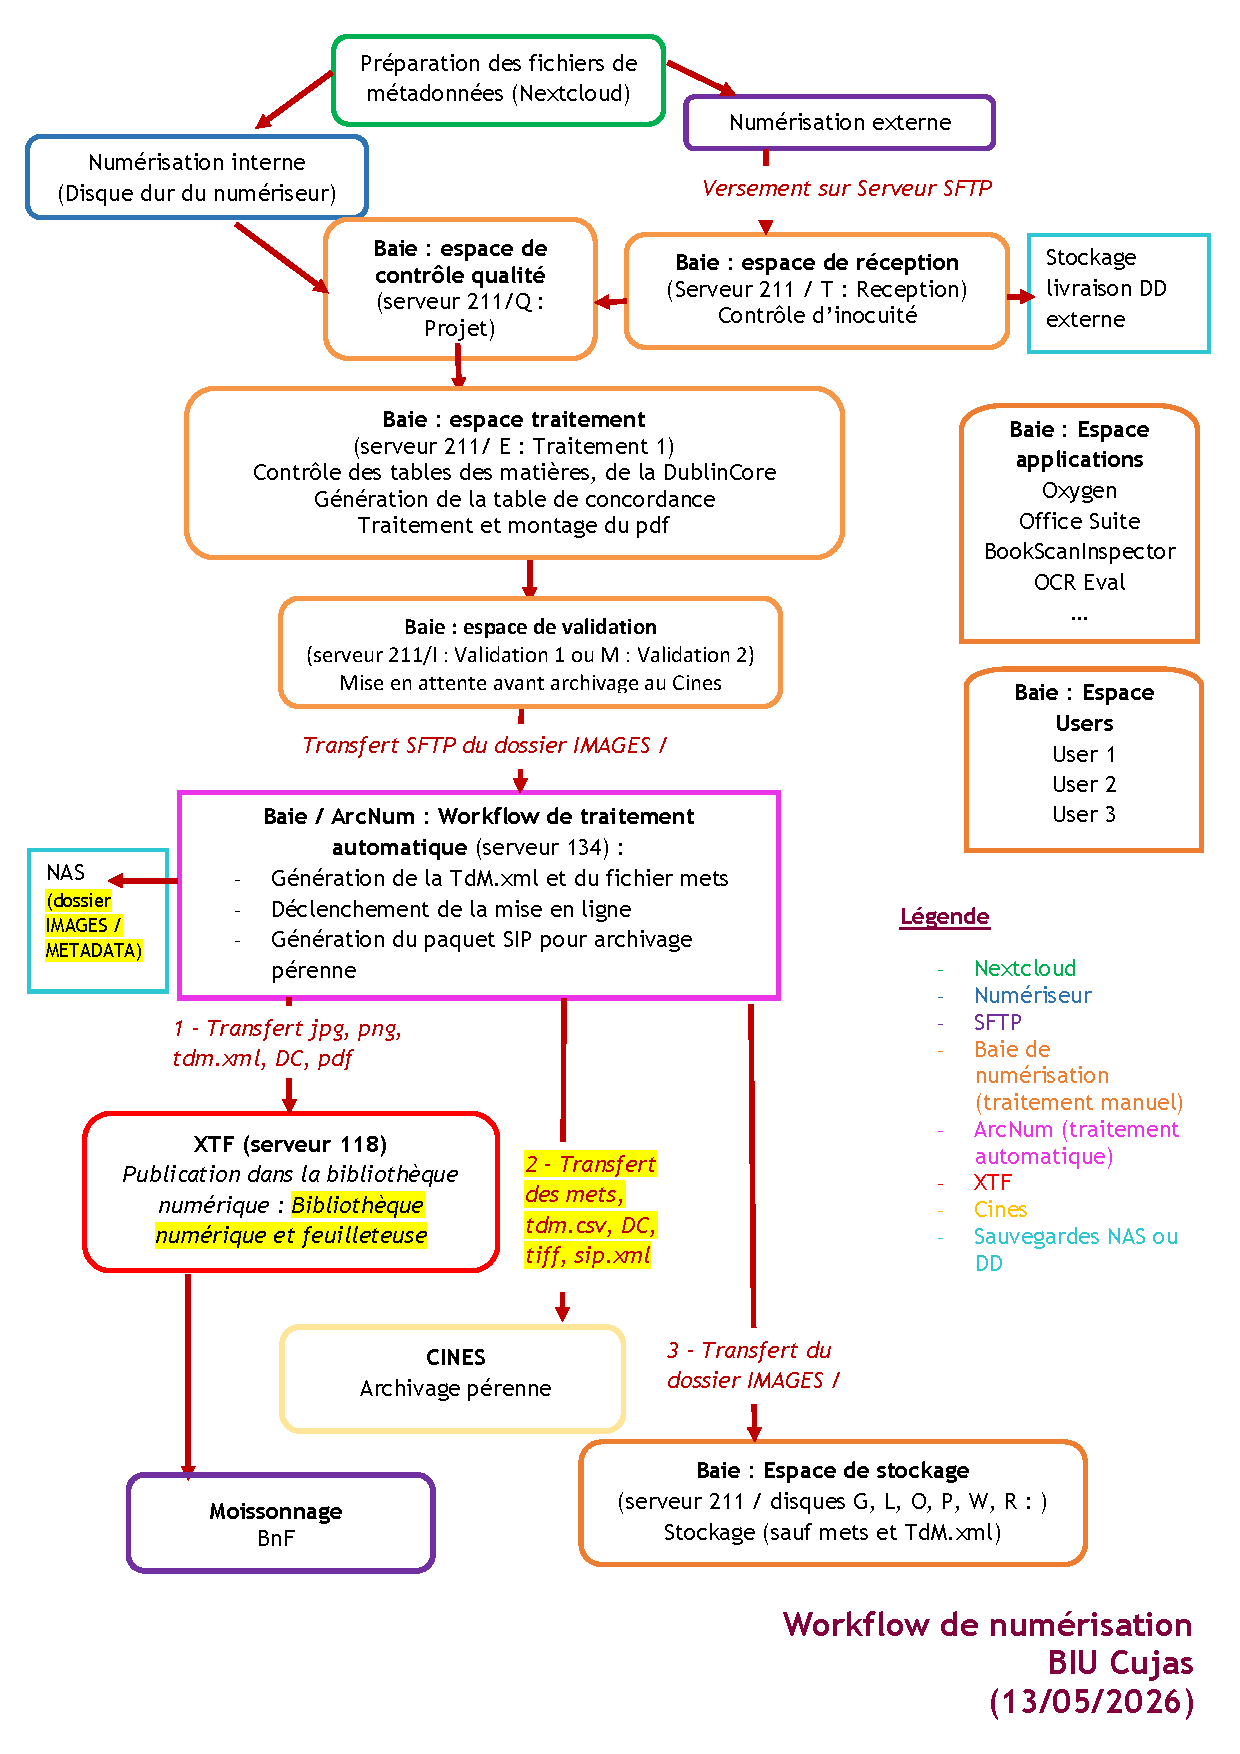
\includegraphics[width=0.5\linewidth]{202605_NUM_schemas_Workflow_prod_publ_V2.pdf}
		\caption{Schéma du workflow de production et de publication}
		\label{fig:workflow_prod_publ}
	\end{figure}

\subsection{Le matériel et le choix des chaînes de production (interne ou externe)}
La mise en œuvre concrète de cette chaîne de production a historiquement reposé sur l'acquisition d'un scanner de marque Kirtas à l'époque du projet Persée. Au-delà des arbitrages scientifiques, la mise en œuvre de la liste \enquote{Pfister-Roumy} se heurte rapidement aux contraintes matérielles de cet appareil. Cet équipement s'avère en effet beaucoup moins efficace que prévu, confrontant les agents à de \enquote{nombreux problèmes liés à son utilisation : il n'est pas possible d'utiliser toutes les fonctions automatiques de numérisation du scanner, forte probabilité de devoir passer en manuel pour les papiers anciens, difficultés de réglage et fréquents dysfonctionnements nécessitant d'éteindre et de rallumer les appareils et de refaire tous les réglages à chaque fois} \footcite{2007RefonteProgramme}. De surcroît, le scanner fait peser un fort risque de dégradation physique sur les documents originaux, dont la fragilité exige d'extrêmes précautions.

Malgré les difficultés logistiques pressenties face à l'ampleur d'un tel projet, l'établissement valide la liste \enquote{Pfister-Roumy} en articulant sa production autour d'une chaîne hybride. D'une part, à la suite de l'exposition virtuelle consacrée à Jean Carbonnier, la Bibliothèque Cujas dispose désormais d'une chaîne de numérisation en interne opérationnelle et prête à être mobilisée. Cette infrastructure s'est d'ailleurs renforcée grâce à la création de la célèbre \enquote{liste Pfister-Roumy}, une campagne de numérisation \enquote{alimentée entièrement en interne grâce aux compétences du département informatique} \footcite{2007RefonteProgramme}. Pour ce corpus, l'établissement fait le choix de traiter en interne exclusivement les \enquote{ouvrages postérieurs à 1830 avec l'océrisation et la relecture partielle sur les parties structurantes} \footcite{2007RefonteProgramme}. D'autre part, pour les documents antérieurs à 1830, la Bibliothèque Cujas privilégie une externalisation de la numérisation auprès d'un partenaire spécialisé, la société Puces et Plumes. Cette décision vise à \enquote{préserver le document}, car l'usage de son propre scanner représente un risque pour ces ouvrages déjà fragiles. Le prestataire se charge de numériser les documents en \enquote{mode image, [et] de faire la saisie fine des tables des matières} \footcite{2007RefonteProgramme}. Cette répartition stratégique du travail permet d'alimenter l'ambitieux projet de créer une bibliothèque numérique juridique fédérée unie par le protocole de moissonnage \ac{OAI-PMH}. Cette liste Pfister-Roumy constitue ainsi le véritable pilier fondateur de la bibliothèque numérique CujasNum.

Aujourd'hui, l'établissement dispose d'un nouveau matériel de numérisation de production récent (scanner de table de haute performance), ce qui permet de s'affranchir de ces contraintes historiques et de réévaluer la répartition entre traitements internes et externes. Le choix d'orienter un document vers la chaîne interne (numérisation sur place par les agents du \ac{DPCN}) ou vers une chaîne externe (prestataires ou chaînes de la \ac{BNF}) se fait désormais de manière stratégique par corpus, selon l'état de conservation physique de l'ouvrage, son format et les volumes à traiter.

\subsection{Le bordereau de numérisation}
Afin de garantir la bonne exécution de la campagne de numérisation, la méthodologie de travail de la Bibliothèque Cujas s'appuie sur l'établissement systématique d'un bordereau constituer de différentes parties. La première partie correspond à la notice bibliographique du document; la seconde détaille précisément sa pagination ainsi que les éventuelles particularités observées, par exemple des pages portant la même pagination; enfin, la dernière partie dresse l'état du document avant le transfert chez le prestataire \footannexe{\nameref{annexe_A_rapport_audit} pour voir l'entretien avec Sandrine Limandri qui détaille la façon dont la bibliothèque Cujas travail}.

\subsection{La phase de traitement: traitement d'images et OCRisation} 
Une fois la numérisation effectuée, la bibliothèque réceptionne les images brutes réalisées sous le format de conservation maître \ac{TIFF}. L'équipe effectue alors \enquote{un contrôle physique, livre en main, pour vérifier la complétude des images et s'assurer qu'aucune page ne manque par rapport au bordereau}\footannexe{\nameref{annexe_A_rapport_audit} pour voir l'entretien avec Sandrine Limandri.}. C'est par la suite qu'un script informatique local permet de générer les formats de diffusion légers (\ac{JPEG}, \ac{PDF}) et de produire automatiquement la table de concordance \enquote{qui fait correspondre chaque numéro d'image à la pagination réelle du livre}\footannexe{\ref{annexe_A_rapport_audit} pour voir l'entretien avec Sandrine Limandri.}. 

Cette orientation technique vers des fichiers statiques découle de la conception originelle de CujasNum, pensée comme \enquote{un simple répertoire \ac{PDF}} calqué sur la structure physique et matérielle d'un livre (volume et pages)\footannexe{\nameref{annexe_A_rapport_audit}.}. Pour dépasser cette contrainte et rendre la consultation des images plus ergonomique, une visionneuse \ac{JPEG} a été implémentée en 2013 pour permettre à l'usager de feuilleter le document de façon dynamique dans son navigateur\footannexe{\nameref{annexe_A_rapport_audit}.}.

\ac{XTF} possède de nombreuses contraintes techniques, l'une d'elles réside dans l'obligation d'avoir le format \ac{PDF} afin de mettre le document en ligne. Le système a été conçu comme \enquote{un simple répertoire \ac{PDF}} calqué sur la structure physique d'un livre (volume et pages)\footannexe{\nameref{annexe_A_rapport_audit}.}. Cela rend donc difficile l'ajout de tout autre types de documents ne respectant pas ce principe. Pour rendre la consultation des images plus agréable, une visionneuse \ac{JPEG} a été implémentée en 2013 pour permettre à l'usager de feuilleter le document de façon dynamique. 

Parallèlement au traitement de l'image, le traitement sémantique et textuel s'organise autour d'une stratégie d'océrisation (\ac{OCR}) différenciée. Au démarrage du traitement numérique, l'\ac{OCR} est appliqué exclusivement aux documents postérieurs à 1830 afin de permettre la recherche plein-texte au sein du texte imprimé\footcite{2011_programmeNumerisationPar}. Pour les ouvrages antérieurs à cette date charnière, la numérisation s'effectue uniquement en mode image pour préserver des supports physiques fragiles. L'absence d'\ac{OCR} sur le corpus de ces textes anciens est palliée par l'enrichissement sémantique de la table des matières, garantissant ainsi une navigation intellectuelle fine dans le document. Tandis que la personne en charge du contrôle qualité valide la conformité des métadonnées du Dublin Core, des moniteurs étudiants se voient confier la saisie intégrale de ces tables des matières sous format Excel/CSV, une tâche indispensable pour restituer fidèlement la structure de l'ouvrage et guider le chercheur\footannexe{\nameref{annexe_A_rapport_audit} pour voir l'entretien avec Sandrine Limandri.}.

\subsection{La phase de publication et d'archivage pérenne}
La validation définitive du contrôle qualité par l'équipe ouvre la voie à la phase finale de publication et d'archivage pérenne. Ce jalon requiert de minutieuses vérifications formelles et sémantiques effectuées par le technicien en charge de la validation. En plus de s'assurer de la conformité requise pour le versement au \ac{CINES}, le technicien doit \enquote{vérifier qu'il y a bien une image pour chaque page} et contrôler que le nommage de chaque fichier image respecte strictement la structure du \enquote{code-barres suivi du numéro d'image et de l'extension}\footannexe{\nameref{annexe_A_rapport_audit}.}. Il lui incombe également de s'assurer que les liens hypertextes figurant dans les métadonnées et commençant par le protocole non sécurisé \enquote{http} soient systématiquement remplacés par des adresses sécurisées \enquote{https} afin de prévenir tout blocage lors de l'ingestion ou de la consultation\footannexe{\nameref{annexe_A_rapport_audit}.}. 

Une fois ces critères formels validés, le protocole impose de contrôler la résolution et le taux de compression des images \ac{JPEG} et \ac{TIFF} à l'aide de l'outil \textit{IrfanView}, de verrouiller les fichiers \ac{PDF} de diffusion grâce à un mot de passe de protection institutionnel, et de valider la conformité de l'arborescence \ac{XML} du schéma de métadonnées Dublin Core afin de conjurer tout risque de rejet lors de l'ingestion par le \ac{CINES}\footcite{2010CRArchivage}. Les données sont ensuite transférées de manière asynchrone via un protocole \ac{SFTP} sécurisé (WinSCP) durant la nuit vers l'espace de publication final\footannexe{\nameref{annexe_A_rapport_audit} pour voir l'entretien avec Mebrouk Leulmi.}. Ce protocole de transfert différé, cloisonné et restreint a été mis en œuvre par le Département informatique technique (\ac{DIT}) à la suite d'une violente tentative d'attaque par rançongiciel subie par l'établissement en 2017, obligeant à sécuriser drastiquement tous les flux réseau entre la baie de traitement locale et les serveurs publics de l'université\footannexe{\nameref{annexe_A_rapport_audit} pour voir l'entretien avec Mebrouk Leulmi.}.

Le second volet de cette phase finale concerne l'archivage pérenne, confié au \ac{CINES}. Pour chaque ouvrage, la bibliothèque compile les fichiers d'images maîtres au format \ac{TIFF} et les fichiers de métadonnées descriptives et de gestion au format \ac{METS} (\textit{Metadata Encoding and Transmission Standard}) et PREMIS au sein d'un paquet de versement d'archives nommé \ac{SIP} (\textit{Submission Information Package})\footcite{2010CRArchivage}\footannexe{\nameref{annexe_A_rapport_audit} pour voir l'entretien avec Mebrouk Leulmi.}. Ce paquet standardisé garantit la préservation à long terme de la matière première numérique contre l'obsolescence matérielle. Néanmoins, ce circuit historique est aujourd'hui fragilisé. Le blocage récent des versements automatiques vers le \ac{CINES} contraint la Bibliothèque Cujas à conserver l'ensemble de ses fichiers intermédiaires au sein de son propre espace de stockage local (un \ac{NAS} de 40 à 50 téraoctets), provoquant une saturation critique de la baie de numérisation\footannexe{\nameref{annexe_A_rapport_audit}.}.

Cette procédure de versement réglementaire s'applique également aux documents dépourvus de structure linéaire, à l'instar du fonds iconographique de l'établissement. Pour répondre aux exigences d'ingestion du \ac{CINES}, les pièces d'images isolées doivent être compilées sous la forme d'un fichier \ac{PDF} unique. Le technicien élabore alors une table des matières et une table de concordance artificielles pour simuler la structure d'un volume physique, tandis qu'un plan d'archivage spécifique est défini conjointement avec les équipes du \ac{CINES} afin de valider ce profil de versement particulier\footannexe{\nameref{annexe_A_rapport_audit}.}.

Une autre particularité liée à la chaîne de numérisation réside dans l'indexation appliquée aux documents numériques de la bibliothèque numérique. C'est l'indexation Hauville qui est créée à partir de l'indexation \ac{RAMEAU}. 
\section{L’indexation propre à la bibliothèque Cujas}
La singularité de la Bibliothèque Cujas réside en grande partie dans l'adoption d'un système d'indexation tout à fait spécifique, peu utilisé et largement méconnu des autres établissements documentaires. La bibliothèque numérique s'appuie en effet sur cette indexation locale, une méthodologie originale qui doit son nom à sa conceptrice, qui a activement collaboré au projet de préfiguration de la première bibliothèque numérique de Cujas. 

Ce choix méthodologique s'explique par le fait qu'à sa création la bibliothèque numérique de Cujas reposait sur des \enquote{mots-clés libres qui généraient des incohérences} documentaires. Pour y remédier, il n'était cependant pas toujours envisageable de recourir au langage standardisé \ac{RAMEAU}, considéré comme inadapté au droit en raison de son caractère trop généraliste \footcite{cecilebolardLindexationPistePour2022}. C'est dans ce contexte que cette indexation a été développée : s'appuyant structurellement sur le référentiel \ac{RAMEAU}, elle ne le mobilise que lorsqu'il s'avère pertinent, mais n'hésite pas à le déconstruire dans le cas contraire afin de proposer des vedettes plus adaptées \footcite{2013_Num_Indexation_manuel_FHdocEspaceTravail}. 

Cette indexation débute par une phase d'analyse documentaire approfondie, au cours de laquelle le catalogueur examine le titre, la table des matières, et la quatrième de couverture, tout en procédant à l'identification des thèmes de l'ouvrage \footcite{2013_Num_Indexation_manuel_FHdocEspaceTravail}. Une fois ces concepts sémantiques identifiés, ils sont traduits dans le langage d'autorité national \ac{RAMEAU}. En l'absence de terme adéquat au sein de ce référentiel, l'établissement s'appuie \enquote{sur une forme normalisée qui est la plus courante comme Wikipédia ou vocabulaire des termes juridiques de Cornu par exemple} afin de combler les lacunes terminologiques du dictionnaire officiel \footcite{2013_Num_Indexation_manuel_FHdocEspaceTravail}. 

À l'issue de cette phase de normalisation, le technicien construit une vedette d'indexation structurée en deux ou trois éléments en fonction de la spécialité du domaine traité. Puis, il construit la vedette pouvant être composé entre deux ou trois éléments en fonction du domaine traité. Cette indexation comprend la vedette de forme (code, travaux préparatoires...), et le concept juridique. L'idée est de pouvoir \enquote{relire la vedette à l'envers en mettant un de ou dans le(s)} \footcite{2013_Num_Indexation_manuel_FHdocEspaceTravail}. Un exemple type de facette pouvant être trouvé sur CujasNum est celle-ci : Eglise -- Administration. Une autre particularité de cette indexation est la possibilité d'avoir \enquote{une indexation à la fois générique et spécifique. Il est possible d'avoir plusieurs vedettes construites ayant des liens de hiérarchie entre elles}, comme par exemple : Droit civil -- Obligations et Droit civil -- Contrats. Cela permet ainsi de mieux guider le lecteur \footcite{2013_Num_Indexation_manuel_FHdocEspaceTravail}.

À l'origine, l'application pratique de cette méthode d'indexation souffre d'un manque d'encadrement normatif au sein de la Bibliothèque Cujas. Il était en effet fréquent qu'elle soit faite par différente personnes, car il s'agissait initialement\enquote{de mots-clés apposés dans les notices Dublin Core}\footcite{2013_Num_Indexation_manuel_FHdocEspaceTravail}. La multiplication des personnes en charge de l'indexation ont rapidement entraîné\enquote{ainsi des incohérences} sémantiques majeures. Certains catalogueurs utilisaient par exemple un simple trait d'union tandis d'autres recouraient au tiret cadratin, une divergence typographique en apparence mineure mais suffisante pour générer artificiellement de nouvelles facettes redondantes et non connectées dans l'indexeur \ac{XTF} \footnote{\ref{annexe_A_rapport_audit}}. Pour pallier cette dérive et homogénéiser le catalogue, la direction impose un cadre strict en exigeant que \enquote{tout le monde indexerait de la même façon, en proposant de recourir à la liste d'autorité \ac{RAMEAU} sur BNOpale}\footcite{2013_Num_Indexation_manuel_FHdocEspaceTravail}.Face à ces difficultés structurelles, la \ac{BNF} recommande de \enquote{faire une liste fermée du vocabulaire utilisé \ac{RAMEAU} tant qu'il n'y a pas trop d'ouvrages numérisés}\footcite{2013_Num_Indexation_manuel_FHdocEspaceTravail}. Si l'astuce fonctionne ponctuellement, elle ne résiste pas au traitement de masse, la \ac{BNF} jugeant la méthode impraticable à l'échelle de plusieurs milliers d'unités. 

Bien que ce dispositif ait initialement été  validé par la \ac{BNF}, cette approbation s'est doublée d'une mise en garde prospective quant à sa pérennité. La \ac{BNF} soulignait en effet qu'un tel système d'autorités commencerait inévitablement à poser de sérieux problèmes de cohérence et de gestion documentaire dès lors que la bibliothèque numérique franchirait le seuil critique des 1 000 documents numérisés \footcite{2013_Num_Indexation_manuel_FHdocEspaceTravail}.

Clé de voûte d'une navigation fluide au sein d'une bibliothèque numérique, l'indexation repose entièrement sur la qualité des métadonnées -- décrites comme les \enquote{garants de fonctionnalités de recherche et de navigation satisfaisantes} \footcite{stutzmannSignalerRessourcesNumerisees2013}. Dès lors, l'interopérabilité des données s'avère cruciale : privée de cette capacité d'échange standardisé, une bibliothèque numérique risque son évincement progressif de la communauté malgré tous les services novateurs que celle-ci peut proposer. C'est précisément à l'aune de ce double impératif de description et d'interconnexion qu'il convient d'analyser les défaillances de l'infrastructure de CujasNum, dont l'obsolescence technique a progressivement transformé l'innovation initiale en une lourde dette technique.
